\documentclass[10pt,conference,twocolumn]{style}
%Use esse arquivo para incluir novos pacotes

\usepackage[%usado para determinar medidas
	top=1.78cm,
	bottom=1.78cm,
	left=1.65cm,
	right=1.65cm,
	headsep=0cm,
	%showframe
]{geometry}
%\usepackage[justification=centering]{caption}
\usepackage{times}
\usepackage{afterpage}
\usepackage{dblfloatfix}
\usepackage{enumitem}%redefinir espacos itemize
\usepackage{graphicx}
\usepackage{longtable}
% \usepackage{url,hyperref}
\usepackage[utf8]{inputenc}
\usepackage{float}%mais controle para manipular figuras
\usepackage{caption}%manipular legenda da figura e tabela
\usepackage{mathtools}%equacoes
\usepackage[hang,flushmargin]{footmisc}
\usepackage{xcolor}
\usepackage{wrapfig} %usado para envolver figura com texto
%\usepackage[portuguese]{babel}
\usepackage{fancyhdr}%criacao do cabecalho
\usepackage{etoolbox}
\usepackage[export]{adjustbox}%mais controle para ajustar tamanho da tabela
\usepackage{comment}%ambiente para comentario
\usepackage{relsize} %usado por comandos \mathlarger
\usepackage{lipsum}

\usepackage{amsmath}  % fórmulas
\usepackage{amsfonts} % símbolos 
\usepackage{amssymb}  % mais símbolos
\usepackage{graphicx} % figuras
\usepackage{booktabs} %tabelas

\usepackage{caption}% http://ctan.org/pkg/caption

%Referencia bibliografica
\usepackage[
	style=numeric, % default: numeric/abnt
	sorting=none,
	maxbibnames=10]{biblatex}
\addbibresource{ref.bib}

%Idioma. Use "english" para trabalhos em inglês
% \usepackage[brazil]{babel}

\usepackage{threeparttable}
\usepackage{fontawesome} % icons

\usepackage{listings}
\usepackage{xcolor}

%Ajustes na legenda da figura. Incluindo espacamento apos a legenda
\captionsetup[figure]{labelformat={default},labelsep=period,font=footnotesize, name=\footnotesize{Fig.},justification=centering,singlelinecheck=false,belowskip=0\normalbaselineskip}
%\pagenumbering{gobble}

%Ajustes na legenda da tabela. 
%\captionsetup[table]{labelformat={default},labelsep=newline,font={sc,footnotesize},justification=centering,singlelinecheck=false}
\captionsetup[table]{format=plain,labelformat=simple,labelsep=period,justification=raggedright,singlelinecheck=false,skip=0pt,font=small}

%\renewcommand{\headrulewidth}{0pt}

\makeatletter
\newcommand{\linebreakand}{%
	\baselineskip
	\end{@IEEEauthorhalign}
	\hfill\mbox{}\par
	\mbox{}\hfill\begin{@IEEEauthorhalign}
}
\makeatother


%%%%%%%%%%%%%%%%%%%%%%%%%%%%%%%%%%%%%%%%%%%%%%%%%%%%%%%%%%%%%%%%%%%%%%%%%
%    Configuracaoes de Idioma
%    Considerando babel = brazil
%%%%%%%%%%%%%%%%%%%%%%%%%%%%%%%%%%%%%%%%%%%%%%%%%%%%%%%%%%%%%%%%%%%%%%%%% 

% \addto\captionsbrazil{
%   \renewcommand{\abstractname}{Abstract}
%   \renewcommand{\figurename}{Figura}
%   \renewcommand{\tablename}{Tabela}
% }
%
% %considerando babel = english
% \addto\captionsenglish{
%   \renewcommand{\tablename}{Table}
% }

% Define custom colors for syntax highlighting
\definecolor{keywordcolor}{rgb}{0.0, 0.0, 1.0} % Blue for keywords
\definecolor{stringcolor}{rgb}{0.0, 0.5, 0.0}  % Green for strings
\definecolor{commentcolor}{rgb}{0.5, 0.5, 0.5} % Gray for comments
\definecolor{backgroundcolor}{rgb}{1, 1, 1} % Light background

% Configure listings style for C code
\lstdefinestyle{mystyle}{
	backgroundcolor=\color{white}, % Set background color
	basicstyle=\ttfamily\footnotesize,       % Font size and type
	keywordstyle=\color{keywordcolor}\bfseries, % Keywords in blue and bold
	stringstyle=\color{stringcolor},          % Strings in green
	commentstyle=\color{commentcolor}\itshape, % Comments in gray and italic
	%numbers=left,                            % Line numbers on the left
	%numberstyle=\tiny\color{gray},           % Style of line numbers
	%stepnumber=1,                            % Line number step
	%numbersep=5pt,                           % Space between line numbers and code
	tabsize=2,                               % Tab size
	breaklines=true                          % Break long lines
}

\bibliography{ref.bib}

\begin{document}

\title{Métodos Numéricos de Zero Real:\\ Teoria, Implementação e Comparação}
\author{
	\IEEEauthorblockN{Gabriel dos Santos Schmitz\\}
	\IEEEauthorblockN{Vitor Augusto Salata de Souza\\}
	\IEEEauthorblockA{RA 2487438 \& 2461200, Engenharia de Computação, \\
		\faEnvelope\ gabrielzschmitz@protonmail.com \\
		\faEnvelope\ vitsou@alunos.utfpr.edu.br \\}
}

\maketitle
\setlength{\textfloatsep}{0pt}  % Reduce space between figure and text
\setlength{\intextsep}{0pt}     % Remove space above/below the figure when inline
\setlength{\floatsep}{0pt}      % Remove space between floats
\section{Introdução}

A busca por zeros de funções é um problema fundamental na matemática aplicada,
engenharia e computação científica. Métodos numéricos desempenham um papel
essencial nessa tarefa, pois muitas funções não possuem soluções analíticas
exatas, tornando necessário o uso de aproximações iterativas.

Neste artigo, exploraremos cinco dos principais algoritmos para encontrar zeros
reais de funções: \textit{Bisseção, Newton-Raphson, Falsa Posição, Ponto Fixo e
Secante}. Cada um desses métodos possui vantagens e limitações, variando em
critérios como taxa de convergência, robustez e eficiência
computacional.\cite{asano2009calculo}

Além de analisar o funcionamento teórico de cada abordagem, desenvolveremos um
programa que permitirá visualizar esses algoritmos em ação. Isso possibilitará
uma compreensão mais intuitiva dos diferentes comportamentos e estratégias
utilizadas para aproximar as raízes de uma função.

Por fim, realizaremos uma comparação detalhada do desempenho de cada método,
avaliando sua eficácia em diferentes cenários. Com essa abordagem, buscamos
oferecer um guia prático e acessível para estudantes, pesquisadores e
profissionais que desejam compreender e aplicar algoritmos de busca de raízes de
forma eficiente.\cite{ruggiero1996calculo}

\section{Fundamentos Teóricos}

Nesta seção, são apresentados os métodos numéricos implementados. Cada método é
descrito em termos de conceito, funcionamento, convergência e
vantagens/desvantagens.\cite{ruggiero1996calculo}~\cite{asano2009calculo}

\subsection{\textbf{Método da Bisseção}}

O método da bisseção é um algoritmo de busca de raízes que divide repetidamente
um intervalo ao meio e seleciona o subintervalo que contém a
raiz.\cite{bartle1983elementos}~\cite{moreira2011curso}

\subsubsection{Funcionamento}

Dada uma função contínua \( f(x) \) e um intervalo \([a, b]\) onde \( f(a) \cdot
f(b) < 0 \), o método calcula o ponto médio \( c = \frac{a + b}{2} \). Se \(
f(c) = 0 \), \( c \) é a raiz. Caso contrário, o intervalo é reduzido para \([a,
		c]\) ou \([c, b]\), dependendo do sinal de \( f(c) \).

\subsubsection{Convergência}

O método converge linearmente, garantindo uma raiz desde que \( f(x) \) seja
contínua no intervalo e haja uma mudança de sinal. O erro absoluto é reduzido
pela metade a cada iteração, e o número de iterações necessárias para atingir
uma precisão \( \epsilon \) é dado por:
\[
	n \geq \frac{\log(b - a) - \log(\epsilon)}{\log(2)}.
\]

\subsubsection{Vantagens e Desvantagens}

\begin{itemize}
	\item \textbf{Vantagens}: Simplicidade e garantia de convergência.
	\item \textbf{Desvantagens}: Convergência lenta comparada a outros métodos.
\end{itemize}

\subsection{\textbf{Método de Newton-Raphson}}

O método de Newton-Raphson é um algoritmo iterativo que usa a derivada da função
para aproximar a raiz.\cite{moreira2011curso}~\cite{bartle2010introduction}

\subsubsection{Funcionamento}

Dada uma função \( f(x) \) e sua derivada \( f'(x) \), o método começa com uma
estimativa inicial \( x_0 \). A cada iteração, a aproximação é atualizada por:
\[
	x_{n+1} = x_n - \frac{f(x_n)}{f'(x_n)}.
\]
O processo repete até que \( |x_{n+1} - x_n| \) seja menor que uma tolerância
pré-definida.

\subsubsection{Convergência}

O método converge quadraticamente, desde que a estimativa inicial seja próxima
da raiz e \( f'(x) \neq 0 \).

\subsubsection{Vantagens e Desvantagens}

\begin{itemize}
	\item \textbf{Vantagens}: Convergência rápida.
	\item \textbf{Desvantagens}: Requer o cálculo da derivada e pode divergir se
	      a estimativa inicial for inadequada.
\end{itemize}

\subsection{\textbf{Método da Falsa Posição (Regula Falsi)}}

O método da falsa posição é uma variação do método da bisseção que usa uma
aproximação linear para estimar a raiz.\cite{bartle1983elementos}

\subsubsection{Funcionamento}

Dada uma função \( f(x) \) e um intervalo \([a, b]\) onde \( f(a) \cdot f(b) < 0
\), o método calcula a interseção da reta que liga \( (a, f(a)) \) e \( (b,
f(b)) \) com o eixo \( x \):
\[
	c = \frac{a \cdot f(b) - b \cdot f(a)}{f(b) - f(a)}.
\]
Se \( f(c) = 0 \), \( c \) é a raiz. Caso contrário, o intervalo é reduzido para
\([a, c]\) ou \([c, b]\), dependendo do sinal de \( f(c) \).

\subsubsection{Convergência}

Mais rápida que a bisseção, mas ainda linear.

\subsubsection{Vantagens e Desvantagens}

\begin{itemize}
	\item \textbf{Vantagens}: Mais eficiente que a bisseção em muitos casos.
	\item \textbf{Desvantagens}: Pode ser lento se a função for muito
	      não-linear.
\end{itemize}

\subsection{\textbf{Método do Ponto Fixo}}

O método do ponto fixo transforma o problema de encontrar a raiz de \( f(x) = 0
\) em encontrar um ponto fixo \( g(x) = x \).\cite{moreira2011curso}

\subsubsection{Funcionamento}

Reescreva \( f(x) = 0 \) como \( x = g(x) \). Escolha uma estimativa inicial \(
x_0 \) e itere:
\[
	x_{n+1} = g(x_n).
\]
O processo repete até que \( |x_{n+1} - x_n| \) seja menor que uma tolerância
pré-definida.

\subsubsection{Convergência}

Depende da escolha de \( g(x) \). A convergência é garantida se \( |g'(x)| < 1
\) em um intervalo contendo a raiz.

\subsubsection{Vantagens e Desvantagens}

\begin{itemize}
	\item \textbf{Vantagens}: Simplicidade e flexibilidade na escolha de \( g(x) \).
	\item \textbf{Desvantagens}: Pode divergir se \( g(x) \) não for adequada.
\end{itemize}

\subsection{\textbf{Método da Secante}}

O método da secante é uma variação do método de Newton que não requer o cálculo
da derivada.\cite{dequadros2009fundamentos}

\subsubsection{Funcionamento}

Dada uma função \( f(x) \) e duas estimativas iniciais \( x_0 \) e \( x_1 \), o
método calcula a próxima aproximação usando a fórmula:
\[
	x_{n+1} = x_n - f(x_n) \cdot \frac{x_n - x_{n-1}}{f(x_n) - f(x_{n-1})}.
\]
O processo repete até que \( |x_{n+1} - x_n| \) seja menor que uma tolerância
pré-definida.

\subsubsection{Convergência}

Superlinear (ordem \( \approx 1.61\)), mas não tão rápida quanto o método de
Newton.

\subsubsection{Vantagens e Desvantagens}

\begin{itemize}
	\item \textbf{Vantagens}: Não precisa do cálculo da derivada.
	\item \textbf{Desvantagens}: Pode divergir se as estimativas iniciais não forem adequadas.
\end{itemize}

\subsection{\textbf{Comparação Geral dos Métodos}}

A Tabela \ref{tab:comparacao} resume as características principais dos métodos
discutidos. \newline

\begin{table}[H]
	\centering
	\begin{longtable}{|p{1.97cm}|p{1.16cm}|p{1.3cm}|p{1.16cm}|p{1cm}|}
		\hline
		\textbf{} \newline \textbf{Método} & \textbf{Tipo} \newline \textbf{Converg.} & \textbf{Deriv.} \newline \textbf{Necessária?} & \textbf{Garantia} \newline \textbf{Converg.} & \textbf{Veloc.} \newline \textbf{Converg.} \\
		\hline
		\endfirsthead
		\hline
		\endfoot
		\hline
		Bisseção                           & Linear                                   & Não                                           & Sim                                          & Lenta                                      \\
		Newton-Raphson                     & Quadrática                               & Sim                                           & Não                                          & Rápida                                     \\
		Falsa Posição                      & Linear                                   & Não                                           & Sim                                          & Moderada                                   \\
		Ponto Fixo                         & Dep. \( g(x) \)                          & Não                                           & Dep. \( g(x) \)                              & Variável                                   \\
		Secante                            & Superlinear                              & Não                                           & Não                                          & Moderada                                   \\
		\hline
	\end{longtable}
	\caption{Comparação dos métodos numéricos.}
	\label{tab:comparacao}
\end{table}

\section{Implementação}

A implementação dos métodos de busca de raízes foi desenvolvida em Python,
utilizando bibliotecas como \texttt{ttkbootstrap} para a interface gráfica e
\texttt{matplotlib} para a visualização dos métodos em ação. O código está
estruturado em três arquivos principais: \texttt{app.py}, \texttt{ui.py} e
\texttt{functions.py}.

\subsection{Visão Geral}

A estrutura do código é organizada da seguinte forma:
\begin{itemize}
	\item \textbf{app.py}: Ponto de entrada da aplicação, responsável por inicializar a interface gráfica.
	\item \textbf{ui.py}: Contém a implementação da interface gráfica e gerencia a interação do usuário.
	\item \textbf{functions.py}: Implementa os métodos numéricos de busca de raízes e fornece suporte para os cálculos.
\end{itemize}

\subsection{Interface}

A interface gráfica do aplicativo foi implementada no arquivo \texttt{ui.py},
utilizando a biblioteca \texttt{ttkbootstrap} para um design moderno e
intuitivo. A interface permite ao usuário inserir uma função \( f(x) \), definir
um intervalo ou chute inicial, escolher um método de busca de raízes e
visualizar os resultados tanto numericamente quanto graficamente.

O código é estruturado em três classes principais:
\begin{itemize}
	\item \textbf{RootFinderUI}: Gerencia a interface principal, incluindo
	      campos de entrada, botões de ação e a exibição dos resultados.
	\item \textbf{PlotManager}: Responsável por gerar e atualizar os gráficos
	      das funções e dos métodos utilizados.
	\item \textbf{ThemeManager}: Permite alternar entre temas claros e escuros
	      para melhor experiência visual.
\end{itemize}

\subsubsection{RootFinderUI: Estrutura da Interface}

A classe \texttt{RootFinderUI} define os elementos principais da interface e
gerencia as interações do usuário. A inicialização ocorre no método
\texttt{\_\_init\_\_}, onde são criados os seguintes componentes:
\begin{itemize}
	\item Campos de entrada para a função \( f(x) \), \( g(x) \) (caso
	      necessário), intervalo \([a, b]\) ou chute inicial e tolerância.
	\item Um menu suspenso para selecionar o método numérico desejado.
	\item Botões para executar a busca da raiz, copiar os resultados, salvar o
	      gráfico e alternar o tema.
	\item Um rótulo para exibir os resultados numéricos.
	\item Uma área gráfica onde a função e a raiz encontrada são plotadas.
\end{itemize}

O trecho de código abaixo demonstra a criação do campo de entrada para a função
\( f(x) \):

\hrule
\lstset{style=mystyle}
\begin{lstlisting}[language=Python]
ttk.Label(input_frame, text="f(x):").grid(row=0, column=0, sticky="w")
self.f_entry = ttk.Entry(input_frame, width=40)
self.f_entry.grid(row=0, column=1, columnspan=3)
self.f_entry.insert(0, "sin(x) + cos(x) + 1")
\end{lstlisting}
\hrule

A entrada padrão para a função é \( f(x) = \sin(x) + \cos(x) + 1 \), podendo ser
alterada pelo usuário.

\subsubsection{Seleção de Método e Ajuste de Parâmetros}

Os métodos disponíveis são carregados automaticamente a partir da classe
\texttt{RootFinderMethods}, permitindo que novos algoritmos sejam adicionados
sem necessidade de modificar a interface:

\hrule
\lstset{style=mystyle}
\begin{lstlisting}[language=Python]
self.methods = self._get_root_finding_methods()
self.method_combobox = ttk.Combobox(
    input_frame, textvariable=self.method_var, values=list(self.methods.keys())
)
\end{lstlisting}
\hrule

A função \texttt{\_get\_root\_finding\_methods} percorre os métodos definidos na
classe \texttt{RootFinderMethods} e os adiciona à interface permitindo
selecionar funções a ignorar.

\subsubsection{Execução do Cálculo e Exibição dos Resultados}

Ao pressionar o botão "Solve", o método \texttt{solve} é chamado, realizando as
seguintes operações:
\begin{enumerate}
	\item Obtém os valores inseridos pelo usuário.
	\item Converte a função de string para código executável usando
	      \texttt{eval}.
	\item Chama o método apropriado de \texttt{RootFinderMethods}.
	\item Exibe a raiz encontrada e o número de iterações.
	\item Atualiza o gráfico com a função e a raiz.
\end{enumerate}

O código abaixo ilustra como a solução é processada:

\hrule
\lstset{style=mystyle}
\begin{lstlisting}[language=Python]
root, iterations, computation_time = self.function_solver.solve(
    f_str, a, b, tol, method_name, g_str
)
result_text = f"Root: {root:.6f}\nIterations: {iterations}\nTime: {computation_time:.6f} s"
self.result_label.config(text=result_text)
\end{lstlisting}
\hrule

Se um erro for encontrado (como ausência de mudanças de sinal no método da
bisseção), uma mensagem de erro é exibida ao usuário.

\subsubsection{Gerenciamento da Visualização Gráfica}

A classe \texttt{PlotManager} é responsável por criar e atualizar os gráficos. O
método \texttt{update\_plot} traça a função no intervalo fornecido e destaca a
raiz encontrada:

\hrule
\lstset{style=mystyle}
\begin{lstlisting}[language=Python]
x = np.linspace(a, b, 400)
y = [self._eval_function(f_str, xi) for xi in x]
self.ax.plot(x, y, label=f"f(x) = {f_str}")
self.ax.scatter([root], [0], color="red", label="Root")
self.ax.axhline(0, color="black", linewidth=0.5)
\end{lstlisting}
\hrule

Além disso, um botão permite salvar o gráfico gerado para análise posterior.

\subsubsection{Personalização da Aparência}

Para melhorar a usabilidade, a classe \texttt{ThemeManager} gerencia os esquemas
de cores do aplicativo. Dois temas estão disponíveis: um claro e um escuro,
alternáveis pelo usuário.

O código abaixo ilustra a alternância de temas:

\hrule
\lstset{style=mystyle}
\begin{lstlisting}[language=Python]
def toggle_theme(self):
    self.current_theme = "minty" if self.current_theme == "darkly" else "darkly"
    self.style.theme_use(self.current_theme)
\end{lstlisting}
\hrule

\subsubsection{Resumo}

A interface do aplicativo proporciona uma experiência interativa e intuitiva
para explorar diferentes métodos numéricos de busca de raízes. Os usuários podem
visualizar o comportamento das funções e comparar a eficiência dos algoritmos de
forma dinâmica.

\subsection{Funções}

Os métodos numéricos utilizados para encontrar raízes de funções foram
implementados no arquivo \texttt{functions.py}. A implementação está organizada
na classe \texttt{RootFinderMethods}, que contém cada método como uma função
estática, permitindo chamadas diretas sem necessidade de instanciar objetos.

Além disso, o módulo inclui a classe \texttt{FunctionSolver}, responsável por
interpretar a função fornecida pelo usuário, selecionar o método adequado e
gerenciar a execução dos cálculos. Essa organização modular facilita a
reutilização e a extensão do código, permitindo adicionar novos métodos sem
impactar a estrutura principal.

A seguir, são detalhadas as implementações de cada método, explicando suas
operações e como os parâmetros de entrada são utilizados para conduzir o
processo iterativo de busca da raiz.

\subsubsection{Bisseção}

A função \texttt{bisection} recebe como entrada uma função \( f \), um intervalo
inicial \([a, b]\), uma tolerância e um número máximo de iterações. O código
inicia verificando se \( f(a) \) e \( f(b) \) possuem sinais opostos. Caso
contrário, uma exceção é levantada.

O loop principal divide o intervalo ao meio repetidamente até que a raiz seja
encontrada dentro da tolerância ou o número máximo de iterações seja atingido. A
cada iteração:

\begin{enumerate}
	\item O ponto médio \( c \) do intervalo é calculado.
	\item Se \( f(c) \) for zero, a raiz foi encontrada.
	\item Caso contrário, o intervalo é reduzido dependendo do sinal de \( f(c) \).
\end{enumerate}

\hrule
\lstset{style=mystyle}
\begin{lstlisting}[language=Python]
@staticmethod
def bisection(f, a, b, tol=1e-6, max_iter=100):
    if f(a) * f(b) >= 0:
        raise ValueError("The function must have opposite signs at the endpoints.")
    iterations = 0
    while (b - a) / 2 > tol and iterations < max_iter:
        c = (a + b) / 2
        if f(c) == 0:
            break
        elif f(c) * f(a) < 0:
            b = c
        else:
            a = c
        iterations += 1
    return (a + b) / 2, iterations
\end{lstlisting}
\hrule

\subsubsection{Newton-Raphson}

A função \texttt{newton\_raphson} recebe uma função \( f \), um chute inicial \(
x_0 \), uma tolerância e um número máximo de iterações. A cada iteração:

\begin{enumerate}
	\item Calcula-se a derivada numérica de \( f \) no ponto atual \( x_0 \).
	\item Se a derivada for muito pequena, o algoritmo para para evitar divisões por valores próximos de zero.
	\item O próximo valor de \( x_0 \) é calculado usando a equação \( x_1 = x_0 - f(x_0) / f'(x_0) \).
\end{enumerate}

O processo continua até que o valor de \( f(x) \) esteja dentro da tolerância ou
que o número máximo de iterações seja atingido.

\hrule
\lstset{style=mystyle}
\begin{lstlisting}[language=Python]
@staticmethod
def newton_raphson(f, x0, tol=1e-6, max_iter=100):
    iterations = 0
    while abs(f(x0)) > tol and iterations < max_iter:
        df = RootFinderMethods.numerical_derivative(f, x0)
        if abs(df) < 1e-10:
            raise ValueError(
                "Derivative is too close to zero. Choose a better interval or initial guess."
            )
        x0 = x0 - f(x0) / df
        iterations += 1
    return x0, iterations
\end{lstlisting}
\hrule

\subsubsection{Falsa Posição}

A função \texttt{false\_position} segue a mesma estrutura da bisseção, mas em
vez de dividir o intervalo ao meio, calcula um novo ponto \( c \) através de
interpolação linear:
\[
	c = b - \frac{f(b) \cdot (b - a)}{f(b) - f(a)}
\]
Esse novo valor é usado para reduzir o intervalo da mesma forma que na bisseção.

\hrule
\lstset{style=mystyle}
\begin{lstlisting}[language=Python]
@staticmethod
def false_position(f, a, b, tol=1e-6, max_iter=100):
    if f(a) * f(b) >= 0:
        raise ValueError("The function must have opposite signs at the endpoints.")
    iterations = 0
    c = a
    while abs(b - a) > tol and iterations < max_iter:
        c = b - f(b) * (b - a) / (f(b) - f(a))
        if abs(f(c)) < tol:
            break
        if f(c) * f(a) < 0:
            b = c
        else:
            a = c
        iterations += 1
    return c, iterations
\end{lstlisting}
\hrule

\subsubsection{Ponto Fixo}

A função \texttt{fixed\_point} recebe como entrada a função iterativa \( g(x)
\), um chute inicial \( x_0 \), uma tolerância e um número máximo de iterações.
A cada iteração, a função \( g(x) \) é aplicada para gerar um novo valor até que
a diferença entre duas iterações consecutivas seja menor do que a tolerância
especificada.

\hrule
\lstset{style=mystyle}
\begin{lstlisting}[language=Python]
@staticmethod
def fixed_point(_, g, x0, tol=1e-6, max_iter=100):
    iterations = 0
    x1 = x0
    while iterations < max_iter:
        x1 = g(x0)  # Aplica a função iterativa g(x)
        if abs(x1 - x0) < tol:
            return x1, iterations
        x0 = x1
        iterations += 1
    raise ValueError("Fixed-point iteration did not converge.")
\end{lstlisting}
\hrule

O código segue os seguintes passos:
\begin{itemize}
	\item A variável \texttt{iterations} inicia em zero e serve como contador de
	      iterações.
	\item O loop \texttt{while} continua até que o número máximo de iterações
	      seja atingido.
	\item A cada iteração, \texttt{x1} recebe o valor gerado por \texttt{g(x0)},
	      atualizando a estimativa da raiz.
	\item O critério de parada verifica se \( |x_1 - x_0| \) é menor do que a
	      tolerância \texttt{tol}, indicando convergência.
	\item Caso o critério de parada seja atendido, a função retorna o valor de
	      \texttt{x1} e o número de iterações realizadas.
	\item Se o método não convergir dentro do limite de iterações, a função
	      lança um erro informando que a iteração falhou.
\end{itemize}

\subsubsection{Secante}

A função \texttt{secant} aproxima a derivada de \( f(x) \) através da equação da
reta que passa pelos pontos \( (x_{n-1}, f(x_{n-1})) \) e \( (x_n, f(x_n)) \):
\[
	x_{n+1} = x_n - f(x_n) \cdot \frac{x_n - x_{n-1}}{f(x_n) - f(x_{n-1})}
\]
Dessa forma, a secante pode ser vista como uma versão do método de
Newton-Raphson que evita a necessidade de calcular a derivada. O algoritmo é
repetido até que o critério de convergência seja atendido.

\hrule
\lstset{style=mystyle}
\begin{lstlisting}[language=Python]
@staticmethod
def secant(f, a, b, tol=1e-6, max_iter=100):
    iterations = 0
    c = b
    while abs(b - a) > tol and iterations < max_iter:
        c = b - f(b) * (b - a) / (f(b) - f(a))
        if abs(f(c)) < tol:
            break
        a = b
        b = c
        iterations += 1
    return c, iterations
\end{lstlisting}
\hrule

\subsubsection{Resumo}

Cada método implementado apresenta características distintas em relação à
convergência e eficiência. As funções são organizadas dentro da classe
\texttt{RootFinderMethods} e podem ser facilmente chamadas a partir do restante
da aplicação.

\subsection{Aplicativo Final}

O código principal está no arquivo \texttt{app.py}, que inicializa a interface
gráfica e permite a execução dos métodos. A Figura~\ref{fig:demonstracao-app}
apresenta uma visualização do aplicativo em funcionamento.

\begin{figure}[H]
	\centering
	\setlength{\fboxsep}{0pt}
	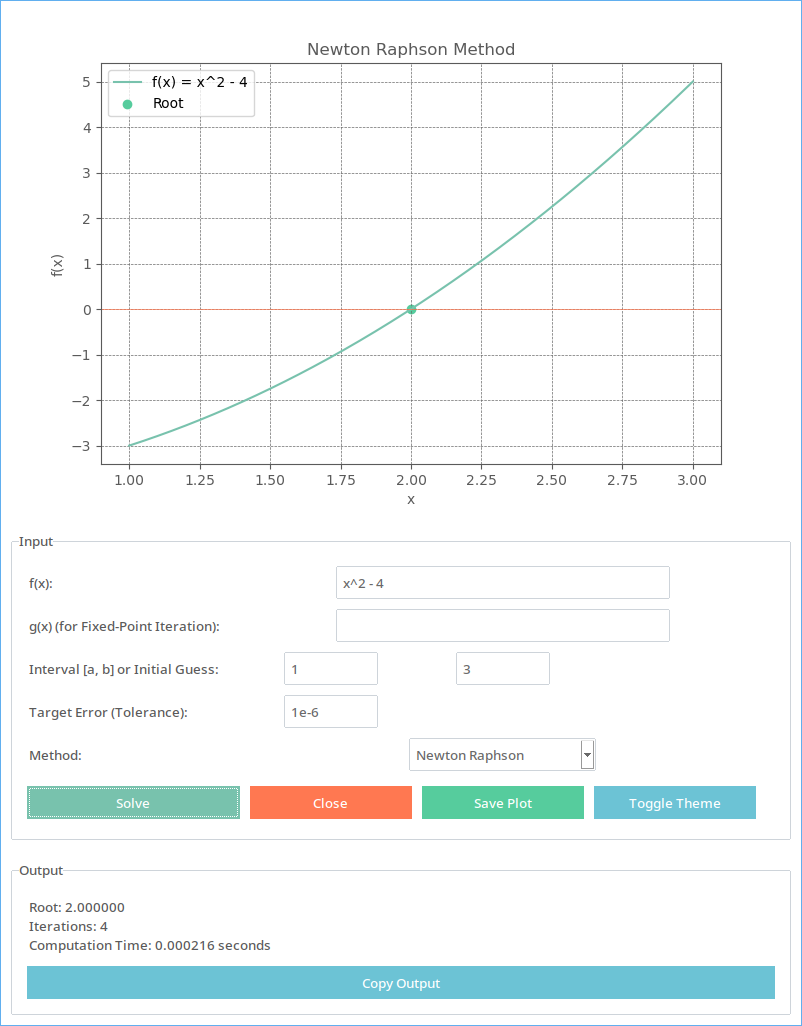
\includegraphics[height=0.5\textwidth]{./fig/demonstracao-app.png}
	\caption{Interface do aplicativo para comparação dos métodos numéricos.}
	\label{fig:demonstracao-app}
\end{figure}

\section{Resultados}

Nesta seção, serão apresentados os resultados dos métodos numéricos aplicados à
função \textbf{\(\boldsymbol{\sin(x) + \cos(x) + 1}\)} com uma tolerância de
\textbf{0,000001}.

\subsection{\textbf{Resultados Gerados Por Cada Método}}

\subsubsection{\textbf{Método da Bisseção}}

Através da utilização do método da bisseção, partindo dos valores iniciais
$[1.1, 3.9]$, chegamos à raiz 3,141592, gerando o seguinte gráfico:

\begin{figure}[H]
	\centering
	\setlength{\fboxsep}{0pt}
	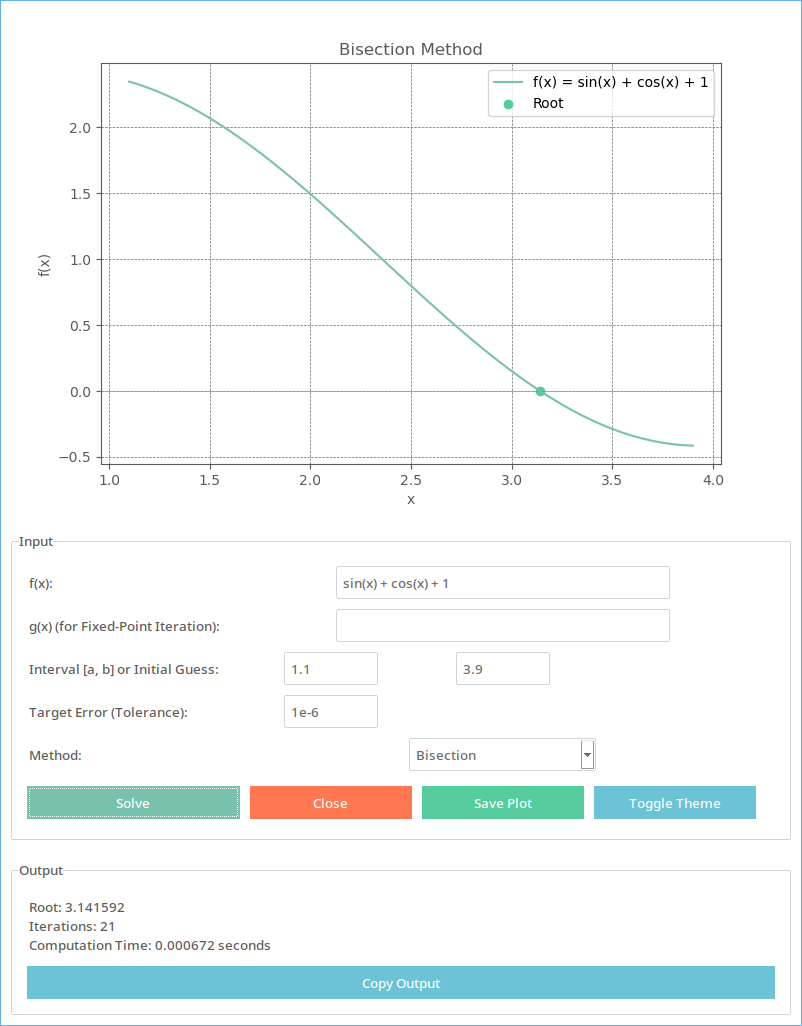
\includegraphics[height=0.5\textwidth]{./fig/bissecao.png}
	\caption{Gráfico da bisseção $[1.1, 3.9]$.}
	\label{fig:grafico-da-bissecao}
\end{figure}

\subsubsection{\textbf{Método de Newton-Raphson}}

Utilizando o método de Newton-Raphson com uma estimativa inicial de $[1.1,
			3.9]$, encontramos a raiz 3,141593 em 8 iterações. O gráfico abaixo ilustra a
convergência do método:

\begin{figure}[H]
	\centering
	\setlength{\fboxsep}{0pt}
	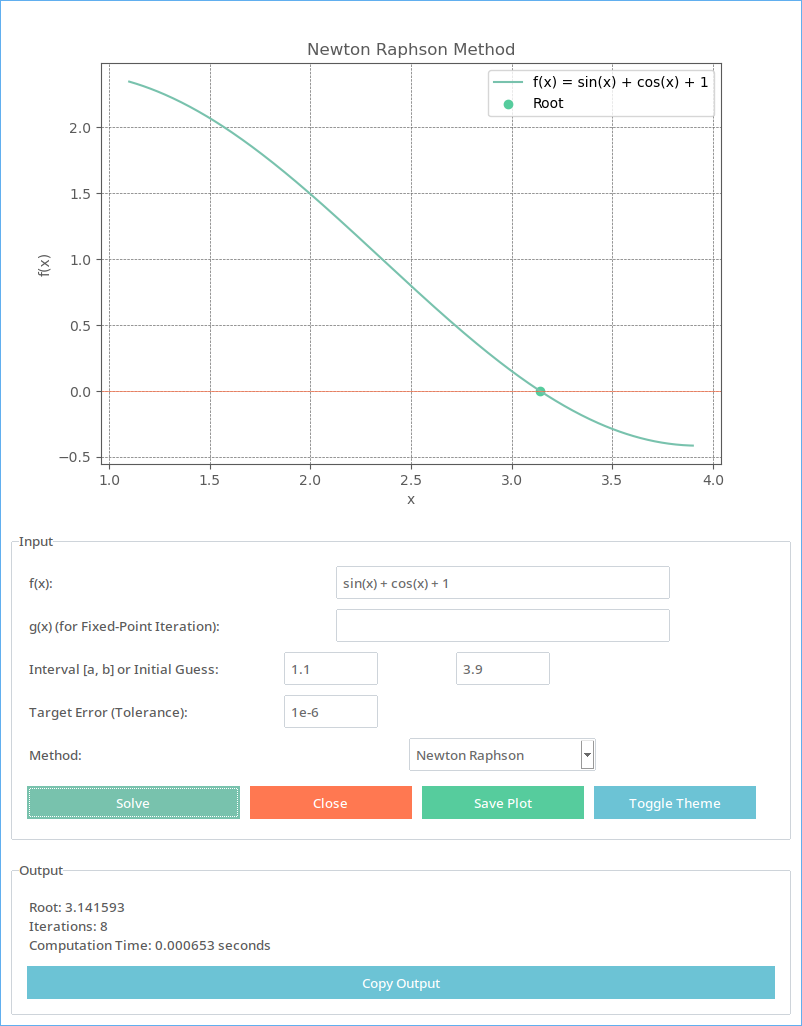
\includegraphics[height=0.5\textwidth]{./fig/newton-raphson.png}
	\caption{Gráfico newton-raphson $[1.1, 3.9]$.}
	\label{fig:grafico-newton-raphson}
\end{figure}

\subsubsection{\textbf{Método da Falsa Posição}}

Com o método da falsa posição, partindo do intervalo $[1.1, 3.9]$, obtivemos a
raiz 3,141593 em 7 iterações. O gráfico a seguir mostra o comportamento do
método:

\begin{figure}[H]
	\centering
	\setlength{\fboxsep}{0pt}
	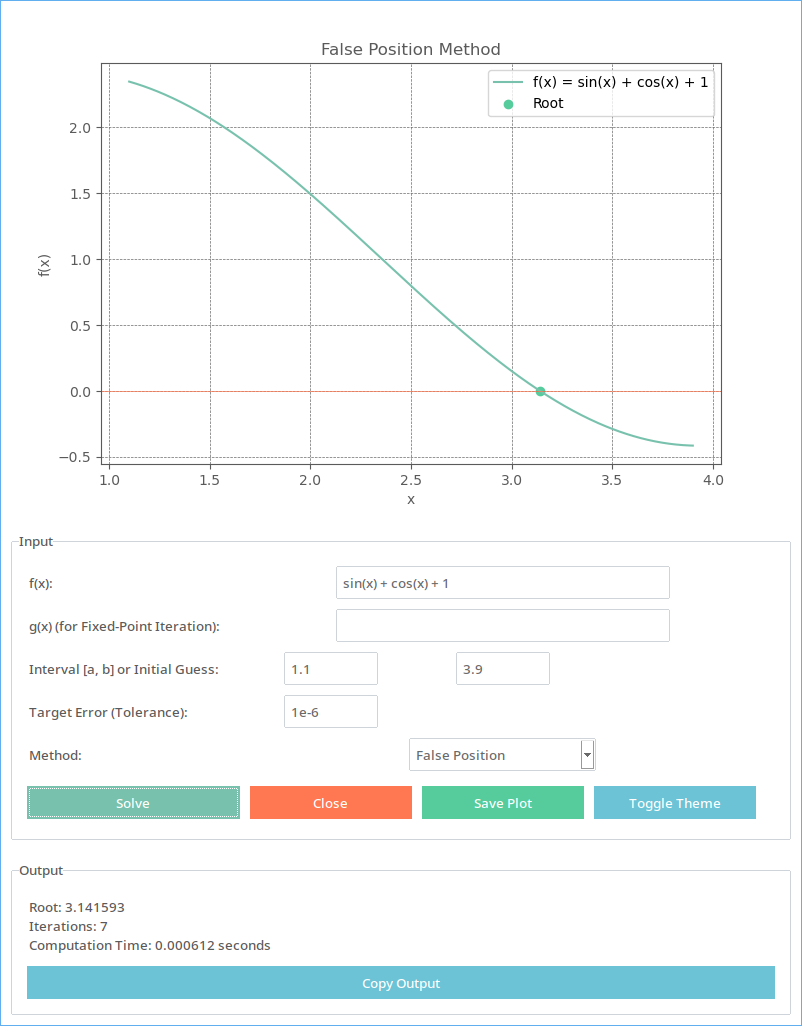
\includegraphics[height=0.5\textwidth]{./fig/ponto-falso.png}
	\caption{Gráfico da falsa posição $[1.1, 3.9]$.}
	\label{fig:grafico-fp}
\end{figure}

\subsubsection{\textbf{Método do Ponto Fixo}}

Aplicando o método do ponto fixo com a função \\ $g(x) = x - 0.5 ⋅ (sin(x) +
	cos(x) + 1)$ e uma estimativa inicial de 1.1, o método convergiu para a raiz
−1,570796 em 20 iterações. O gráfico abaixo ilustra a convergência:

\begin{figure}[H]
	\centering
	\setlength{\fboxsep}{0pt}
	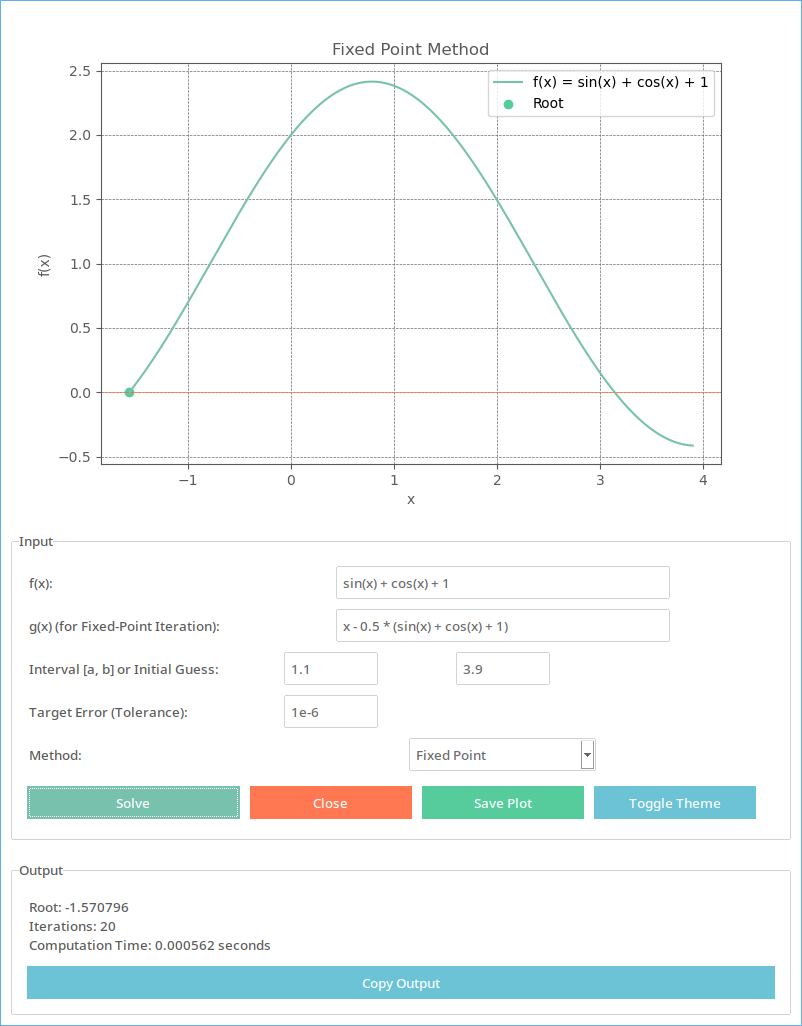
\includegraphics[height=0.5\textwidth]{./fig/ponto-fixo.png}
	\caption{Gráfico do ponto fixo $[1.1, 3.9]$.}
	\label{fig:grafico-pf}
\end{figure}

\subsubsection{\textbf{Método da Secante}}
Por fim, utilizando o método da secante com as estimativas iniciais 1.1 e 3.9,
encontramos a raiz
3,141593 em 6 iterações. O gráfico a seguir mostra a convergência do método:

\begin{figure}[H]
	\centering
	\setlength{\fboxsep}{0pt}
	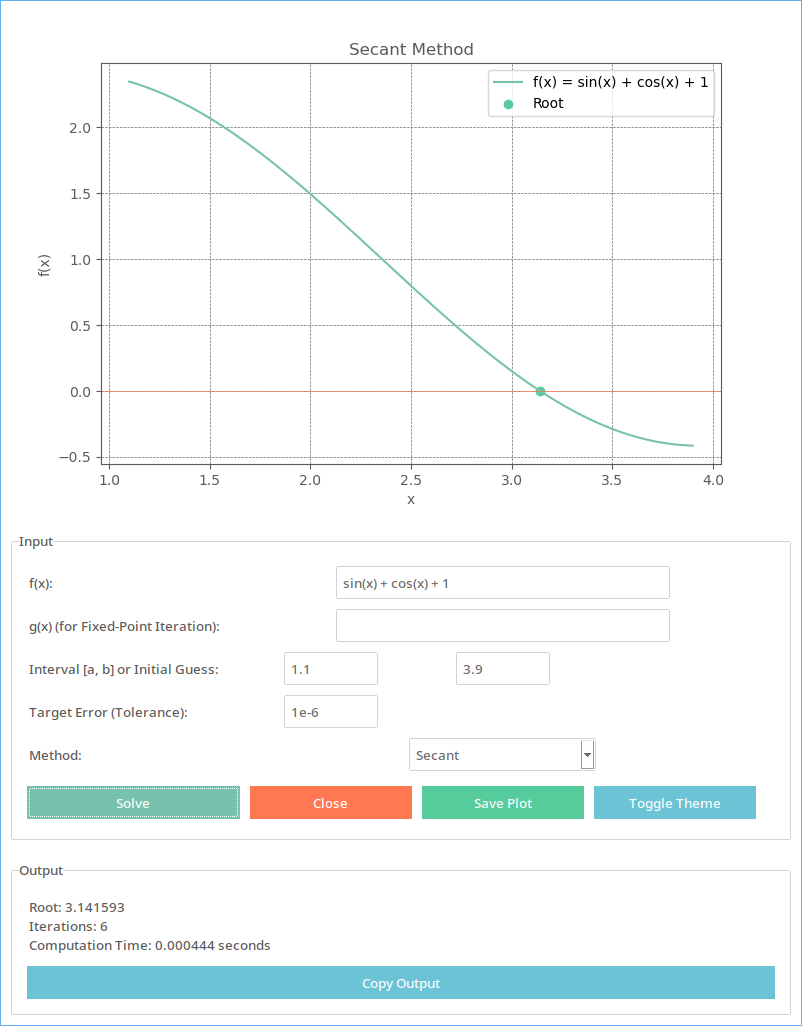
\includegraphics[height=0.5\textwidth]{./fig/secante.png}
	\caption{Gráfico da secante $[1.1, 3.9]$.}
	\label{fig:grafico-sec}
\end{figure}


\begin{figure*}[htbp]
	\centering
	\setlength{\fboxsep}{0pt}
	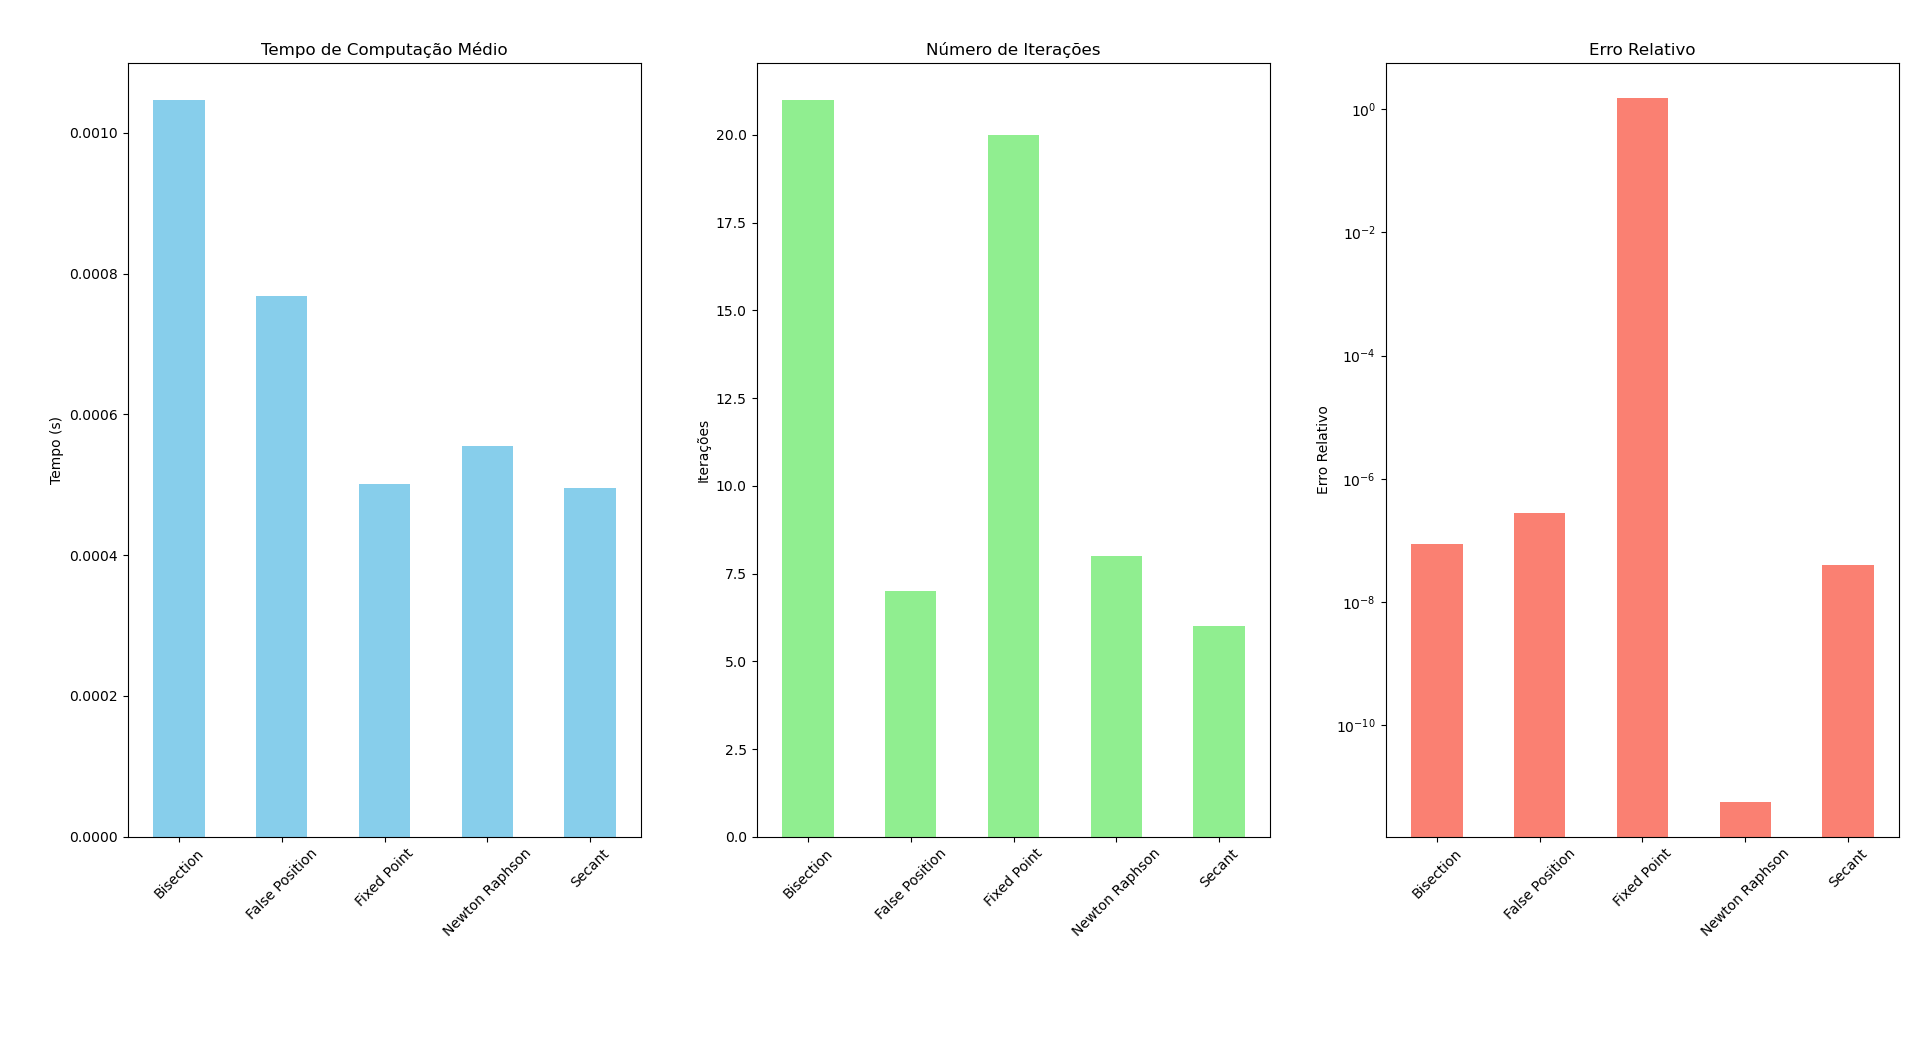
\includegraphics[width=\textwidth]{./fig/benchmark.png}
	\caption{Gráfico comparativo $[1.1, 3.9]$.}
	\label{fig:grafico-comp}
\end{figure*}

\subsection{\textbf{Análise e Comparação}}

Dessa forma, é realizada uma análise comparativa dos métodos numéricos aplicados
à função $f(x) = sin(x) + cos(x) + 1$, considerando o tempo de computação, o
número de iterações e o erro relativo. O gráfico resume os dados
obtidos.\cite{ruggiero1996calculo}~\cite{asano2009calculo}.

Observando de forma geral, é notório como o modo de Newton-Raphson
definitivamente é um dos métodos mais eficientes, devido a seu tempo de execução
satisfatório e baixo erro relativo. Diferentemente do método da bisseção, que
gastou muito tempo de execução e um número muito alto de
iterações.\cite{dequadros2009fundamentos}~\cite{moreira2011curso}.

\subsection{\textbf{Limitações}}

Embora os métodos numéricos sejam ferramentas poderosas para encontrar raízes de
funções, cada um deles possui limitações que devem ser consideradas ao escolher
a abordagem mais adequada para um problema específico. Alguns métodos exigem um
número muito elevado de iterações para atingir a precisão desejada (bisseção),
enquanto outros necessitam de valores iniciais adequados para garantir a
convergência (Newton e secante). Além disso, funções altamente não lineares
podem ser um empecilho para determinados métodos (posição falsa e bisseção), e
uma má escolha da função $g(x)$ pode ser um grande problema para o método do
ponto fixo.\cite{marins1996localizacao}~\cite{lobao_introducao}.

Assim, a junção de todas essas limitações acaba restringindo o desempenho do
software, especialmente quando utilizado por alguém que não domina os
conhecimentos necessários de cálculo numérico, o que pode resultar em resultados
imprecisos.\cite{anton2014calculo}~\cite{bartle1983elementos}.

\section{Conclusão}

Através dos resultados apresentados nesta seção, foi possível comparar a
eficiência e a precisão dos métodos numéricos estudados, considerando o
\textit{tempo de computação}, o \textit{número de iterações} e o \textit{erro
relativo médio}. A fundamentação teórica para esses métodos pode ser encontrada
em \cite{bartle1983elementos} e \cite{ruggiero1996calculo}, que abordam os
princípios matemáticos subjacentes.

Em termos de tempo de computação, o método de Ponto Fixo foi o mais eficiente,
com um tempo médio de $0.000501$ segundos, seguido de perto pelo método Secante,
com $0.000496$ segundos. Por outro lado, o método Bisseção apresentou o maior
tempo médio de execução, com $0.001047$ segundos, embora ainda dentro de limites
aceitáveis para a maioria das aplicações. Esses tempos são ilustrados no gráfico
de \textit{Tempo de Computação Médio} mostrado na Figura \ref{fig:grafico-comp}.

Quanto ao número de iterações, o método de Ponto Fixo também apresentou um
número elevado de iterações ($20$), sendo superado apenas pelo método Bisseção,
que alcançou $21$ iterações. Já os métodos Secante e Newton-Raphson foram os
mais rápidos, com uma média de $6$ e $8$ iterações, respectivamente. Esse
desempenho pode ser observado no gráfico de \textit{Número de Iterações} da
Figura \ref{fig:grafico-comp}.\cite{rudin1976principles}.

Em relação ao erro relativo, os métodos Newton-Raphson e Secante se destacaram
pela precisão, com erros relativos muito baixos ($5.747333e-12$ e
$4.001674e-08$, respectivamente). Em contrapartida, o método de Ponto Fixo
apresentou um erro relativamente alto de $1.500000e+00$, indicando que, apesar
de ser eficiente em termos de tempo, pode não ser adequado para problemas que
exijam alta precisão. O gráfico de \textit{Erro Relativo} na Figura
\ref{fig:grafico-comp} ilustra claramente essas diferenças.

Portanto, pode-se concluir que os métodos Secante e Newton-Raphson são, em
geral, os mais eficientes e precisos, especialmente para problemas que exigem
alta precisão em um número reduzido de iterações. No entanto, a escolha do
método ideal depende das características do problema em questão, como a precisão
desejada e os recursos computacionais
disponíveis.\cite{anton2014calculo}~\cite{dequadros2009fundamentos}.


\setlength{\bibitemsep}{10pt}
\clearpage
\onecolumn
\printbibliography

\end{document}
